\chapter{Grundlagen}
\label{chap:grundlagen}

\section{Fortlaufendes Beispiel}
\label{sec:grundlagen:beispiel}

% Beispiel einleiten
Eine einheitliche und fortlaufende Problemstellung soll der Arbeit als Grundlage dienen. Die Problemstellung besteht aus einem Modell und einem Satz von Testdaten. Alle im weiteren Verlauf diskutierten Modellierungsvarianten werden  diese Problemstellung umsetzen und die Testdaten modellieren.  

	\subsection{Voraussetzungen}
	\label{sec:grundlagen:beispiel:voaussetzungen}

	Der Schwerpunkt der Modellierung liegt bei der Darstellung von Beziehungen zwischen Entit�ten. Dabei soll die
	Problemstellung einerseits nicht zu komplex sein, damit sie �berschaubar bleibt. Andererseits soll sie komplex genug
	sein, um m�glichst alle Bezeihungensarten zwischen Entit�ten abzudecken.

	Die Testdaten sollten so gew�hlt werden, dass idealerweise f�r alle Tests die selben Daten verwendet werden k�nnen.
	Einheitiche Daten sorgen daf�r, dass sich der Entwickler (verbessern) nicht bei verschiedenen Tests in unterschiedliche
	Testdaten hineinversetzten muss. Nur in Ausnahmef�llen sollten Tests modifizierte oder eigene Testdaten verwenden.
	Um dem Entwickler entgegen zu kommen, sollte der Umfang der Testdaten nicht gr��er sein als erforderlich.

	\subsection{Gew�hlte Problemstellung}
	\label{sec:grundlagen:beispiel:gewaehlte_problemstellung}
	Das gew�hlte Beispiel stellt eine starke Vereinfachung des Pr�fungswesens an Hochschulen dar. Auf eine praxisnahe
	Umsetzung wird zugunsten der Komplexit�t verzichtet. Es beinhaltet die folgenden vier Entit�ten:

	\begin{itemize}
		\item \textbf{Professor}: Ein Professor leitet Lehrveranstaltugnen.
		\item \textbf{Lehrveranstaltung}: Eine Lehrveranstaltng wird von einem Professor geleitet. Es kann zu jeder
			Lehrveranstaltung eine Pr�fung geben.
		\item \textbf{Pr�fung}: Eine Pr�fung ist einer Lehrveranstaltung zugeordnet. Au�erdem hat mindestens ein Pofessor
			Aufsicht.
		\item \textbf{Student}: Studenten k�nnen an Lehrveranstaltungen und an Pr�fungen teilnehmen. Studenten haben au�erdem 
			die M�glichkeit, Tutoren von Lehrveranstaltugen zu sein.
	\end{itemize}

	Die Beziehungen der Entit�ten stellen sich wie folgt dar: Eine Lehrveranstaltung muss von genau einem Professor
	geleitet werden, ein Professor kann beliebig viele (also auch keine) Lehrveranstaltungen leiten. Eine Pr�fung ist genau
	einer Lehrveranstaltung zugeordnet. Eine Lehrveranstaltung kann mehrere Pr�fungen haben (z.B. Nachschreibepr�fung).
	Eine Pr�fung muss mindestens von einem Professor beaufsichtigt werden, ein Professor kann in beliebig vielen Pr�fungen
	Aufsicht haben. Jeder Student kann beliebig vielen Lehrveranstaltungen besuchen und Lehrveranstalungen von beliebig
	vielen Studenten besucht werden. Die gleiche Bezeihung gilt f�r Tutoren: Jeder Student kann bei beliebig vielen
	Lehrveranstaltungen Tutor sein und jede Lehrveranstaltung kann beliebig viele Tutoren haben. Schlie�lich kann jeder
	Student auch an beliebig vielen Pr�fungen teilnehmen und umgekehrt eine Pr�fung von einer beliebigen Anzahl von
	Studenten geschrieben werden.

	Abbildung \ref{img:example_er} stellt die Problemstellung grafisch dar. Die Abbildung zeigt, dass es keine 1:1
	Beziehung gibt. Eine 1:1-Beziehung kann jedoch als Spezialfall einer 1:n-Beziehung angesehen werden.

	\begin{figure}[H]
		\centering
		 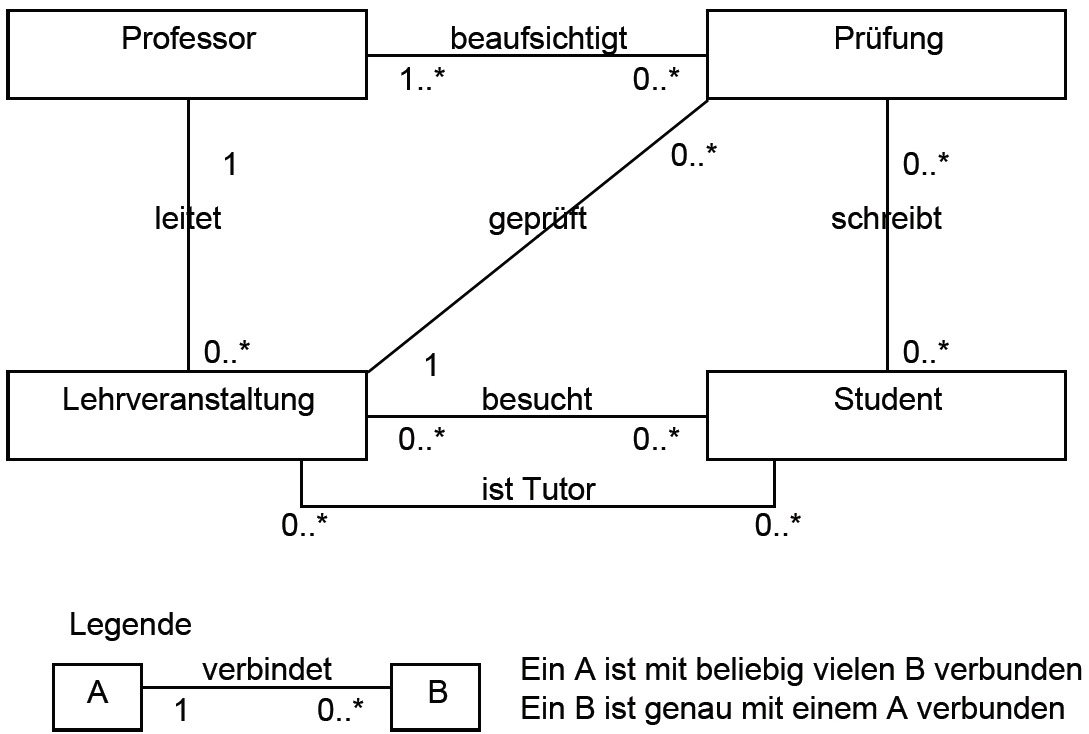
\includegraphics[width=0.8\textwidth]{images/grundlagen/example_hochschule_er.pdf}
		\caption{ER-Diagramm des fortlaufenden Beispiels}\label{img:example_er}
	\end{figure}

	Das entsprechende relationale Modell sieht folgenderma�en aus:
	\begin{figure}[H]
		\centering
		 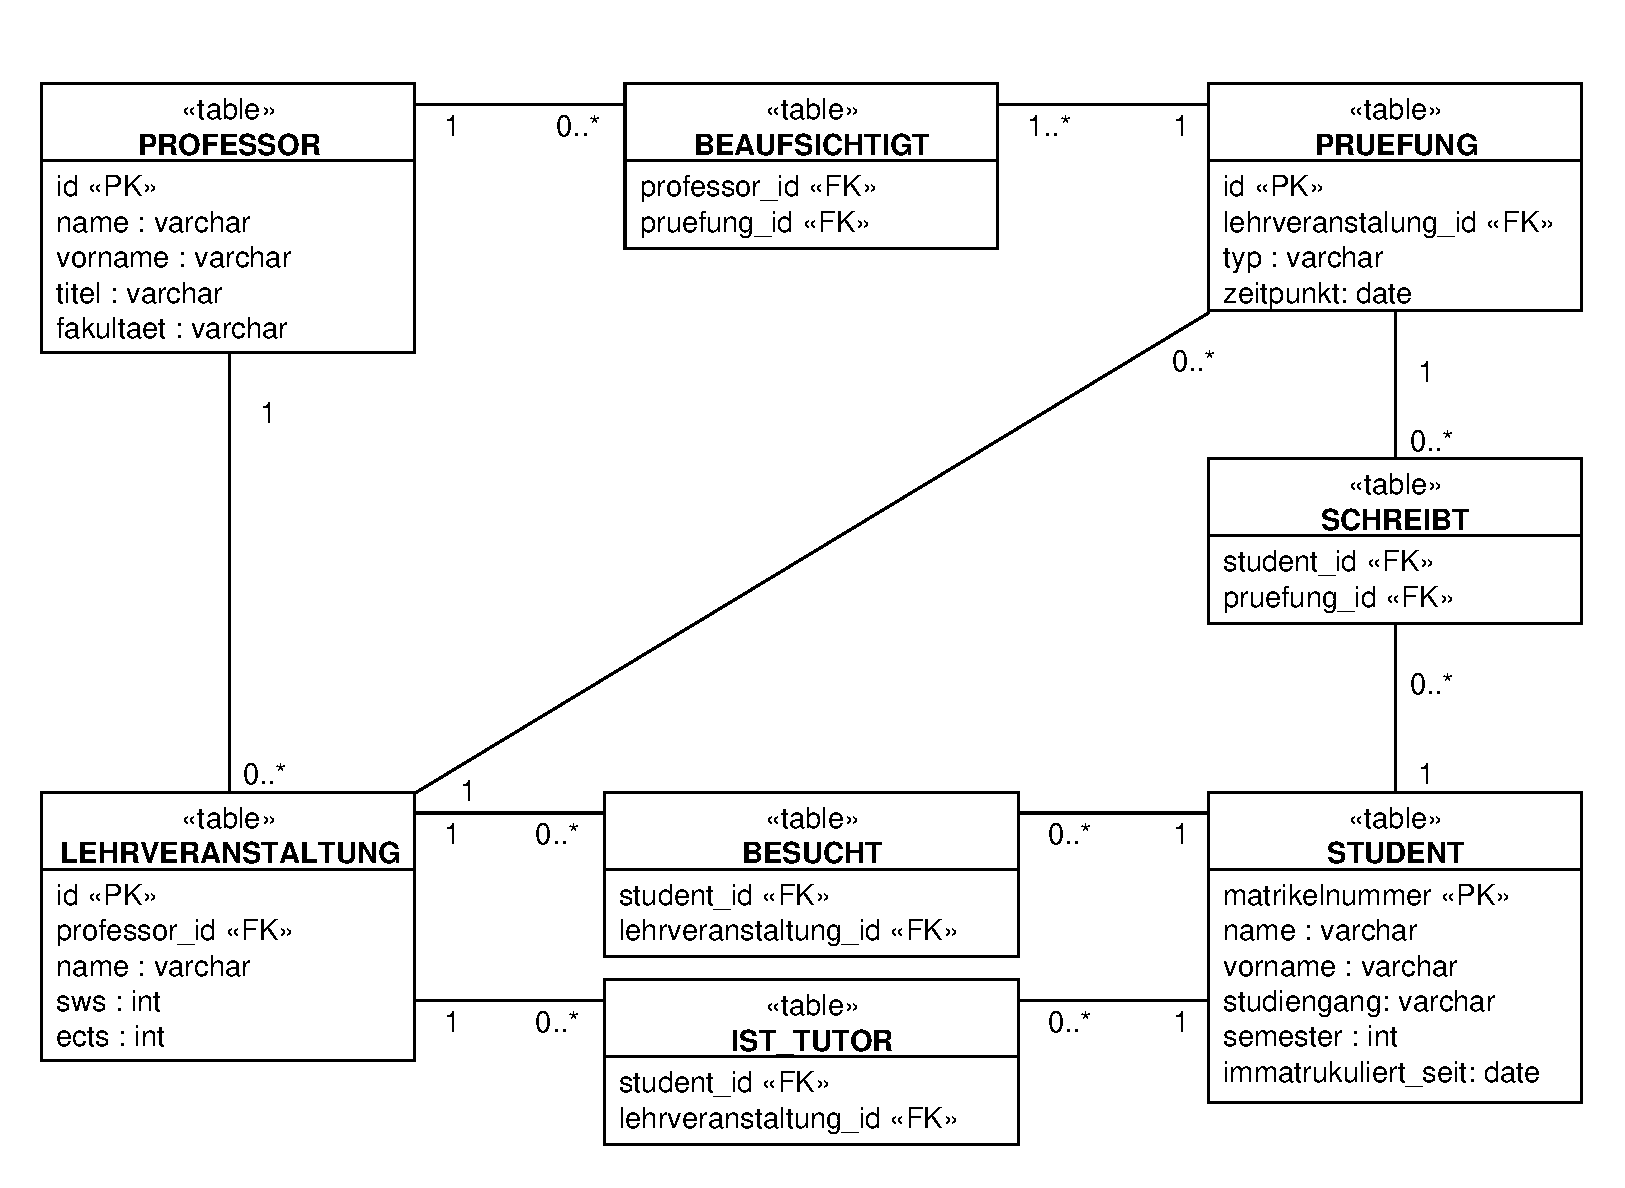
\includegraphics[width=0.95\textwidth]{images/grundlagen/example_hochschule_relational.pdf}
		\caption{Relationales Modell des fortlaufenden Beispiels}\label{img:example_relational}
	\end{figure}

	\subsection{Wahl der Testdaten}
	\label{sec:grundlagen:beispiel:testdaten}

	Um den einen Kompromiss f�r die Komplexit�t der Testdaten zu finden, werden vier Fragestellungen definiert. Diese
	Fragen sollen dabei helfen, den Umfang der Testdaten bestimmen zu k�nnen. Die Fragen stellen sich wie folgt dar:

	\begin{enumerate}
		\item Welcher Professor unterrichtet die meisten Studenten?
		\item Welcher Student nimmt an den meisten Pr�fungen teil?
		\item Welcher Student ist Tutor und nimmt gleichzeitig an der Pr�fung teil?
		\item Welcher Professor macht die wenigste Aufsicht in Fremdveranstaltungen (Lehrveranstaltungen eines anderen
			Professors)?
	\end{enumerate}


\section{Modellierung der Testdaten in DBUnit}

	\subsection{XML Dataset}

	\lstSetXML
	\begin{lstlisting}[caption=XML Dataset, label=listing:xmldataset]
<!DOCTYPE dataset SYSTEM "dataset.dtd">
<dataset>
  <table name="professor">
	  <column>ID</column>
    <column>name</column>
    <row>
      <value>1</value>
      <value>J�rgen W�sch</value>
    </row>
    <row>
      <value>2</value>
      <value>Oliver Haase</value>
    </row>
    </table>
    <table name="lehrveranstaltung">
    <column>ID</column>
    <column>professorID</column>
    <column>name</column>
    <row>
      <value>1</value>
      <value>2</value>
      <value>Verteilte Systeme</value>
    </row>
    <row>
      <value>2</value>
      <value>2</value>
      <value>Concurrency and Design Patterns</value>
    </row>
  </table>
	\end{lstlisting}

	\subsection{Java Dataset}

	\lstSetJava
	\begin{lstlisting}[caption=Java Dataset, label=listing:javadataset]
DefaultTable professor = new DefaultTable(
    "professor",
    new Column[] { 
      new Column("id", DataType.INTEGER),
      new Column("name", DataType.VARCHAR),
		}
  );
professor.addRow(new Object[] { 
    Parameters.Professor.WAESCH_ID,
    "J�rgen W�sch" 
  });
professor.addRow(new Object[] { 
    Parameters.Professor.HAASE_ID,
    "Oliver Haase"
  });
dataSet.addTable(professor);

DefaultTable lehrveranstaltung = new DefaultTable(
    "lehrveranstaltung", 
    new Column[] {
      new Column("id", DataType.INTEGER),
      new Column("professorid", DataType.INTEGER),
      new Column("name", DataType.VARCHAR), 
    }
  );
lehrveranstaltung.addRow(new Object[] {
    Parameters.Lehrveranstaltung.VERTEILTE_SYSTEME_ID,
    Parameters.Professor.HAASE_ID, 
		"Verteilte Systeme" 
  });
lehrveranstaltung.addRow(new Object[] {
    Parameters.Lehrveranstaltung.DESIGN_PATTERNS_ID,
    Parameters.Professor.HAASE_ID,
    "Concurrency and Design Patterns" 
  });
dataSet.addTable(lehrveranstaltung);
	\end{lstlisting}


	\subsection{SB Testing DSL}

	\begin{lstlisting}[caption=SB Testing Dataset (1), label=listing:sbtestingdataset_old]
table_Professor
  .insertRow()
	   .setId(Parameters.Professor.HAASE_ID)
     .setName("Oliver Haase")
	.insertRow()
    .setId(Parameters.Professor.WAESCH_ID)
    .setName("J�rgen W�sch");
	
table_Lehrveranstaltung
  .insertRow()
    .setId(Parameters.Lehrveranstaltung.VERTEILTE_SYSTEME_ID)
    .setProfessorId(Parameters.Professor.HAASE_ID)
    .setName("Verteilte Systeme")
  .insertRow()
    .setId(Parameters.Lehrveranstaltung.DESIGN_PATTERNS_ID)
    .setProfessorId(Parameters.Professor.HAASE_ID)
    .setName("Design Patterns");	
	\end{lstlisting}


\section{Anforderungen an die DSL}

Die Testdaten sollen in einer \textit{Domain Specific Language} (DSL) beschrieben werden. 


\subsection{Zielgruppe}



